\documentclass[10pt]{article}

%% Packages
\usepackage[margin=1in, top=0.75in]{geometry}
\usepackage[utf8]{inputenc}
\usepackage[T1]{fontenc}
\usepackage[usenames,dvipsnames]{xcolor}
\usepackage{amssymb, amsfonts, amsmath, mathrsfs, enumitem, tcolorbox, bbm, graphicx, fullpage, parskip, mathtools, float, amsthm}
\usepackage{tikz,sgame,bbm,todonotes, setspace, soul, array}
\usepackage[english]{babel}
\usepackage{pdfpages}
\setcounter{tocdepth}{3}
% Links (and references)
\definecolor{linkblue}{RGB}{40, 50, 200}
\usepackage[colorlinks=true, allcolors={linkblue}]{hyperref}

%% Math operators
\newcommand*{\ones}{\text{\usefont{U}{bbold}{m}{n}1}}
\newcommand{\reals}{\mathbb{R}}
\newcommand{\rationals}{\mathbb{Q}}
\newcommand{\integers}{\mathbb{Z}}
\newcommand{\naturals}{\mathbb{N}}
\newcommand{\complex}{\mathbb{C}}
\newcommand{\normal}{\mathcal{N}}

% General math
\newcommand{\abs}[1]{\mathop{\left|#1\right|}} % absolute value
\newcommand{\inv}{^{-1}} % inverse
\let\oldST\st
\newcommand{\strikethrough}{\oldST}
\renewcommand{\st}{\;\text{s.t.}\;} % math operator for "such that"
\newcommand{\eg}{\emph{e.g.} }
\newcommand{\ie}{\emph{i.e.} }
\newcommand{\interior}{\mathop{\rm int}}

% Optimization
\newcommand{\argmax}{\mathop{\rm argmax}}
\newcommand{\argmin}{\mathop{\rm argmin}}
\newcommand{\opt}{^\star}
% Analysis, vector spaces, and topology
\newcommand{\set}[1]{\left\{#1\right\}} % set notation
\newcommand{\seq}[1]{_{#1}^{\infty}} % add sequence notiation to set (or to a summation symbol for series)
\newcommand{\setless}{\mathop{\backslash}} % A \ B notation
\newcommand{\pow}{\mathop{\mathcal{P}}} % power set
\newcommand{\im}{\mathop{\rm im}} % image
\newcommand{\spans}{\mathop{\rm span}} % span
\newcommand{\rank}{\mathop{\rm rank}} % rank
\newcommand{\topo}{\mathop{\mathcal{T}}} % topology
\newcommand{\cont}{\mathop{\bf C}} % continuously differentiable

% Matrices
\newcommand\colvector[1]{\begin{bmatrix}#1\end{bmatrix}}
\newcommand\rowvector[1]{\begin{bmatrix}#1\end{bmatrix}}
\newcommand\matrixc[1]{\begin{bmatrix}#1\end{bmatrix}}
\newcommand\matrixp[1]{\begin{pmatrix}#1\end{pmatrix}}
\newcommand\detmatrix[1]{\begin{vmatrix}#1\end{vmatrix}}
\newcommand\rankmatrix{\begin{bmatrix}I_r & \rvline & \mathbf{0}_1\\\hline \mathbf{0}_2 & \rvline & \mathbf{0}_3 \end{bmatrix}}

% Statistics
\newcommand{\cov}{\mathop{\rm cov}} % covariance
\newcommand{\corr}{\mathop{\rm corr}} % correlation
\newcommand{\expect}{\mathop{\mathbb{E}}} % expectation
\newcommand{\indep}{\perp \hspace{-1.4ex} \perp} % independence symbol
\newcommand{\distiid}{\mathop{\overset{\text{i.i.d.}}\sim}} % i.i.d.
\newcommand{\oversim}[1]{\mathop{\overset{\text{#1}}\sim}} % general text over \sim
\newcommand{\prob}{\mathbb{P}}
\newcommand{\mse}{\mathop{\rm MSE}}
\newcommand{\var}{\mathop{\rm Var}}
\newcommand{\sd}{\mathop{\rm sd}}
\newcommand{\se}{\mathop{\rm se}}
\newcommand{\bias}{\mathop{\rm bias}}
\newcommand{\toprob}{\overset{p}{\to}}
\newcommand{\toas}{\overset{a.s.}{\to}}
\newcommand{\todist}{\overset{d}{\to}}
\newcommand{\hyp}{\mathbb{H}}

% Economics
\newcommand{\choice}{\mathop{C_{\succsim}}} % choice correspondence

% Update existing operators
\let\oldExists\exists
\renewcommand{\exists}{\oldExists\;}
\let\oldForall\forall
\renewcommand{\forall}{\;\oldForall\;}
\let\oldEmptyset\emptyset
\renewcommand{\emptyset}{\mathop{\varnothing}}
\newcommand{\parl}{\left(}
\newcommand{\parr}{\right)}
\newcommand{\midbar}{\middle|}
\newcommand{\barl}{\left[}
\newcommand{\barr}{\right]}
\newcommand{\curll}{\left\{}
\newcommand{\curlr}{\right\}}


%% Presentation environments
% Proofs, counterexamples, and disproofs
\renewcommand\qedsymbol{$\openbox$}
\renewenvironment{proof}{{\raggedright \textit{\textbf{Proof.}}}}{\qed} % Proof
\newenvironment{pf}{\begin{proof}}{\end{proof}} % Proof (shorthand)

\newenvironment{disproof}{{\raggedright \textit{\textbf{Disproof.}}}}{$\qed$} % Disproof
\newenvironment{counterex}{{\raggedright \textit{\textbf{Counterexample.}}}}{} % Counterexample

% Theorem styles
\theoremstyle{plain}
\newtheorem{result}{Result}
\newtheorem{lemma}{Lemma}[section]

\newtheorem{theorem}{Theorem}[section]
\newtheorem{proposition}{Proposition}[section]
\newtheorem{corollary}{Corollary}[section]
\newtheorem{axiom}{Axiom}[section]
\theoremstyle{definition}
\newtheorem*{example}{Example}
\newtheorem*{definition}{Definition}
\newtheorem*{exercise}{Exercise}
\newtheorem*{model}{Model}
\newtheorem*{proposition*}{Proposition}
\newtheorem*{model*}{Model}
\newtheorem*{solution}{Solution}
\newtheorem*{remark}{Remark}
\newtheorem*{question}{Question}
\newtheorem*{answer}{Answer}
\newtheorem*{algorithm}{Algorithm}
\newtheorem{assumption}{Assumption}[section]

\newcommand{\blue}[1]{\textcolor{blue}{\emph{#1}}}
\newcommand{\red}[1]{\textcolor{red}{\emph{#1}}}




\newcommand{\gabe}[1]{\todo[inline,color=green!20!white]{\textbf{GS:} #1}}


%% Header
\makeatletter
\newcommand{\course}[1]{\def\@course{#1}}
\newcommand{\term}[1]{\def\@term{#1}}
\renewcommand{\title}[1]{\def\@entitle{#1}}
\renewcommand{\maketitle}{
    \begin{tcolorbox}[colframe=darkgray]
        \begin{center}
            \textbf{\@course} \\[0.25em]
            {\Large\textit{\@entitle}} \\[0.5em]
            \@author \\[0.5em]
            \@term
        \end{center}
    \end{tcolorbox}
    \vspace{1em}
}
\makeatother


%% Code
\usepackage{listings}
\usepackage{beramono}
\lstdefinelanguage{Julia}%
  {morekeywords={abstract,break,case,catch,const,continue,do,else,elseif,%
      end,export,false,for,function,immutable,import,importall,if,in,%
      macro,module,otherwise,quote,return,switch,true,try,type,typealias,%
      using,while},%
   sensitive=true,%
   alsoother={$},%
   morecomment=[l]\#,%
   morecomment=[n]{\#=}{=\#},%
   morestring=[s]{"}{"},%
   morestring=[m]{'}{'},%
   breaklines=true,%
}[keywords,comments,strings]%

\lstset{%
    language         = Julia,
    basicstyle       = \ttfamily,
    keywordstyle     = \bfseries\color{blue},
    stringstyle      = \color{magenta},
    commentstyle     = \color{ForestGreen},
    showstringspaces = false,
}






\title{Game Theory TA Section Notes}
\author{Gabe Sekeres}
\course{ECON 6110}
\term{Spring 2025}

\singlespacing

\begin{document}
\maketitle

\tableofcontents
\newpage

\section{Jan 24}

\subsection{Review}

We introduced the concept of the game, which consists of players, their action sets, and their utility functions.

\begin{definition}
	We have $N=\{1,\dots,n\} \subset \naturals$, $A_i = $ set of actions for player $i$, $A = \bigtimes_{i=1}^n A_i = \prod_{i=1}^n A_i$ is the Cartesian product of the action sets -- $a \in A$, $a = (a_1,\dots,a_n)$.
\end{definition}
\begin{definition}
	A mixed strategy is $\alpha_i: A_i \to [0,1]$ such that $\sum_{a_i \in A_i} \alpha_i (a_i) = 1$. We call the set of these elements $\Delta(A_i)$, where $a_i \in \Delta(A_i)$ is a degenerate distribution. We can say that the Cartesian product $\bigtimes_{i=1}^n \Delta(A_i) = \prod_{i=1}^n \Delta( A_i)$ is the set of profiles of actions, where $\alpha = (\alpha_1,\dots,\alpha_n) \in \bigtimes_{i=1}^n \Delta(A_i)$
\end{definition}
\begin{remark}
	We will often write $\alpha_i(U) = \alpha_i(D) = \frac{1}{2}$, or similar things. We can also write $\alpha_i = \frac{1}{2}U+\frac{1}{2}D$.
\end{remark}
\begin{remark}
	Note the difference between $\prod_{i=1}^n \Delta(A_i)$ and $\Delta\parl\prod_{i=1}^n A_i\parr = \Delta(A)$. Consider an example with two players, where $A_1 = \{U,D\}$ and $A_2 = \{L,R\}$ for $n = 2$. A mixed strategy $\alpha = (\alpha_1,\alpha_2) = (pU + (1-p)D,qL+(1-q)R)$. A specific $\alpha$ is an element of $\prod_{i=1}^n \Delta(A_i)$. If we look at what actually happens in this game, we have
	\[
	\begin{array}{|c|c|c|}
		\hline
		& \underbrace{L}_q &\underbrace{R}_{1-q} \\
		\hline 
		U \Big\} \;p\;\;\;\;\; & pq & p(1-q) \\
		\hline
		D \Big\} \; 1-p & (1-p)q & (1-p)(1-q) \\\hline
	\end{array}
	\]
	However, the other version -- $\Delta\parl\prod_{i=1}^n A_i\parr = \Delta(A)$ -- is the set $\Delta(\{(U,L),(U,R),(D,L),(D,R)\})$, so players 1 and 2 have \emph{correlated probabilities}! The two are not the same at all! The first contains elements of the form
	\[
	pq(U,L) + p(1-q)(U,R) + (1-p)q(D,L) + (1-p)(1-q)(D,R)
	\]
	while the second has elements of the form
	\[
	p_1(U,L) + p_2(U,R) + p_3(D,L) + (1-p_1-p_2-p_3)(D,R)
	\]
	The second can recreate any outcomes in the first, because the first has an additional independence assumption. That may make sense in some contexts, but it's especially restrictive in this context.
\end{remark}
\begin{definition}
	A Mixed Nash Equilibrium can be defined as a pure equilibrium in the mixed extension of the pure game. Mixed equilibria can also be defined as follows: A profile $\alpha\opt := (\alpha_1\opt,\dots,\alpha_n\opt)$ such that for all $i \in N$,
	\[
	U_i(\alpha\opt_i,\alpha_{-i}\opt) \ge U_i(\alpha_i, \alpha_{-i}\opt)
	\]
	for all $\alpha_i \in \Delta(A_i)$.
\end{definition}
\begin{definition}
	The expected utility function \[U_i(\alpha) = \sum_{a \in A} u_i(a_1,\dots,a_n) \cdot \alpha_1(a_1) \cdot \cdots \cdot \alpha_n(a_n)\]
	In continuous space, this generalizes to
	\[
	U_i(\alpha) = \int u_i(a) f(a)da
	\]
	where $f(a)$ is the joint probability density function of $a = (a_1,\dots,a_n)$. Moreover, if we care only about player $i$ (\ie if we are keeping all other players fixed), we have
	\[
	U_i(\alpha) = \sum_{a_i \in A_i} U_i(a_i, \alpha_{-i}) \cdot \alpha_i(a_i)
	\]
\end{definition}
\begin{definition}
	The support of $\alpha_i$ is
	\[
	\supp(\alpha_i) = \{a_i \in A_i : \alpha_i(a_i) > 0\}
	\]
\end{definition}
\begin{proposition}
	If $\alpha\opt$ is a Nash equilibrium, then 
	\[
	U_i(a_i\opt,\alpha_{-i}\opt) = U_i(\alpha_i\opt,\alpha_{-i}\opt)
	\]
	for all $a_i\opt \in \supp(\alpha_i\opt)$.
\end{proposition}
\begin{proof} Notice that
	\[U_i(\alpha_i\opt,\alpha\opt_{-i}) = \sum_{a_i \in A_i} U_i(a_i,\alpha\opt_{-i}) \alpha_i\opt(a_i)\] FSOC assume that $U_i(a_i\opt,\alpha_{-i}\opt) \ne U_i(\alpha_i\opt,\alpha_{-i}\opt)$, so $\exists a_i \in \supp(\alpha_i\opt)$ such that $U_i(a_i,\alpha_{-i}\opt) < U_i(\alpha_i\opt,\alpha_{-i}\opt)$. Then from the summation being a convex combination, dropping $a_i$ from the mixture and increasing weights on other probabilities will strictly increase expected utility, contradicts the assumption that $\alpha\opt$ is Nash. The same holds if the inequality is strict in the other direction, putting more weight on the action in question. Thus, it must be the case that $U_i(a_i\opt,\alpha_{-i}\opt) = U_i(\alpha_i\opt,\alpha_{-i}\opt)$
\end{proof}

\begin{remark}
	This proposition is extremely useful for solving for mixed equilibria.
\end{remark}

\begin{example}
	\red{Matching Pennies} 
	\[
	\begin{array}{|c|c|c|}
		\hline & H & T \\\hline 
		H & (1,-1) & (-1,1) \\\hline
		T & (-1,1) & (1,-1) \\\hline
	\end{array}
	\]
	If we are mixing, where column player chooses $H$ with probability $q$ and row player chooses $H$ with probability $p$, we must have that the expected utilities are equal. Let's go from the row player's perspective:
	\[
	1 \cdot q + (-1)\cdot (1-q) = -1 \cdot q + 1 \cdot (1-q) \Longrightarrow q = \frac{1}{2}
	\]
	So the only $q$ that would make row player indifferent is $\frac{1}{2}$, which works similarly in the other direction.
\end{example}

\begin{proposition}
	For any $\alpha = (\alpha_i,\alpha_{-i})$, the following are equivalent:
	\begin{enumerate}
		\item $\forall \alpha_i' \in \Delta(A_i)$, $U_i(\alpha_i,\alpha_{-i}) \ge U_i(\alpha_i',\alpha_{-i})$
		\item $\forall a_i \in \supp(\alpha_i)$, $\forall \alpha_i' \in \Delta(A_i)$, $U_i(a_i,\alpha_{-i}) \ge U_i(\alpha_i',\alpha_{-i})$
		\item $\forall a_i \in \supp(\alpha_i)$,$\forall a_i' \in A_i$,, $U_i(a_i,\alpha_{-i}) \ge U_i(a_i',\alpha_{-i})$
	\end{enumerate}
\end{proposition}
\begin{proof}
	(Sketch) (1) $\Longrightarrow$(2) from Proposition 1.1, (2) $\Longrightarrow$ (1) by weighted sum, (2) $\Longrightarrow$ (3) clear by set sizes, and (3) $\Longrightarrow$ (2) by weighted sum.
\end{proof}

\section{Jan 31}

\subsection{Review}

\begin{definition}
	A correlated equilibrium (CE) of a game $\langle N, \{A_i\},\{u\}\rangle$ consists of \begin{enumerate}
		\item A finite probability space $(\Omega,\pi)$ (set of states and probability measure on those states) \item For each player $i$, a partition $\mathcal{P}_i$ of $\Omega$ \item For each player $i$, a strategy $\sigma_i : \Omega \to A_i$ with $\sigma_i(\omega) = \sigma_i(\omega')$ whenever $\omega,\omega' \in P_j$ for some $P_j \in \mathcal{P}_i$
	\end{enumerate}
	Such that for every $i \in N$ and any alternative strategy $\tau_i: \Omega \to A_i$ of player $i$ that satisfies $\tau_i(\omega)=\tau_i(\omega')$ whenever $\omega,\omega' \in P_j$ for some $P_j \in \mathcal{P}_i$, we have
	\begin{equation}
		\sum_{\omega \in \Omega}\pi(\omega) u_i(\sigma_i(\omega),\sigma_{-i}(\omega)) \ge \sum_{\omega \in \Omega}\pi(\omega) u_i(\tau_i(\omega),\sigma_{-i}(\omega))
	\end{equation}
	or for all $P_i \in \mathcal{P}_i$,
	\begin{equation}
		\sum_{\omega \in \Omega} \prob(\omega \mid P_i) u_i(\sigma_i(\omega),\sigma_{-i}(\omega)) \ge\sum_{\omega \in \Omega} \prob(\omega \mid P_i) u_i(\tau_i(\omega),\sigma_{-i}(\omega))
	\end{equation}
\end{definition}

\begin{proposition}
	$(1) \Longleftrightarrow (2)$
\end{proposition}
\begin{proof}
	$(\Rightarrow)$ FSOC, assume that $\exists P_i$ such that (2) doesn't hold (so there is $\bar{\tau}_i \succ \sigma_i$ in $P_i$). Then, if we construct $\tau_i(\omega) = \sigma_i(\omega) \forall \omega \not\in P_i$, and $\tau_i(\omega') = \bar{\tau}_i(\omega') \forall \omega' \in P_i$. Then summing, we get a contradiction of (1).
	
	$(\Leftarrow)$ Law of total expectations, we can simply sum over all $P_i$.
\end{proof}

\begin{proposition}
	WLOG, we can assume $\Omega = A = \prod_i A_i = \bigtimes_i A_i$, $\mathcal{P}_i$ consists of sets of the type $\{a \in A: a_i = b_i$ for some action $b_i \in A_i$, and $\sigma_i(a) = a_i$.
\end{proposition}

\begin{remark}
	The construction $\pi$ will give the final distribution of outcomes if the construction is successful.
\end{remark}
\begin{remark}
	The probability space and partitions are engogenous, part of the equilibrium definition.
\end{remark}
\begin{remark}
	Correlated equilibria can be found with linear programming. When all players in the game are no-SWAP regret algorithms, play converges to a correlated equilibrium.
\end{remark}

\subsection{Exercises}

In the following game, compute all of the Nash equilibria and then find a correlated equilibrium that is not in the convex hull of the set of Nash equilibria.
\[
\begin{array}{|c|c|c|}
	\hline & L & R \\\hline
	U & 8,8 & 4,9 \\\hline
	D & 9,4 & 1,1 \\\hline
\end{array}
\]
There are two pure strategy equilibria: $(D,L)$ and $(U,R)$. There are no mixed strategy equilibria: If $c$ plays $L$ with probability $p$, we need that \[U(U,p) = 8p + 4(1-p) = 9p + 1(1-p) = U(D,p) \Longrightarrow p = \frac{4}{3}\]This can never be met, so $r$ is never indifferent, so they will never mix. The game is symmetric, so $c$ will also never mix.

Consider the following correlation structure. The underlying state is $\Omega = \{x,y,z\}$, where $\pi(x) = \pi(y) = \pi(z) = \frac{1}{3}$. Player $r$ partitions this $P^r_1 = \{x,y\},P^r_2 = \{z\}$, and player $c$ partitions this $P^c_1 = \{x\},P^c_2 = \{y,z\}$. The following is an equilibrium: Player $r$ plays $D$ if $\{z\}$ and $U$ if $\{x,y\}$, and Player $c$ plays $R$ if $\{x\}$ and $L$ if $\{y,z\}$. This meets the existence conditions of the correlated equilibrium, but we need to check incentive compatibility. We have that for $r$, if they see $\{z\}$, they know $c$ will play $L$ so they will play $D$ to maximize. If they see $\{x,y\}$, they believe that $c$ will play $R$ with probability $\frac{1}{2}$ and $L$ otherwise, so they attain the highest expected utility by playing $U$. The game is symmetric, so the same holds for $c$. Thus, this is a correlated equilibrium.


\section{Feb 7}

\subsection{Review}

\begin{definition}
	A belief of player $i$ is a probability measure over the set $A_{-i}$, which we denote by $\Delta(A_{-i})$.
\end{definition}

\begin{definition}
	An action $a_i$ of player $i$ in a strategic game is a never-best response if for all beliefs $\mu_i$ there exists $\alpha_i \in \Delta(A_{i})$ such that \[u_i(\alpha_i,\mu_i) > u_i(a_i,\mu_i)\]This means that for every belief of player $i$ there is \emph{some} action that is better for player $i$ than $a_{i}$.
\end{definition}

\begin{definition}
	An action $a_i$ of player $i$ in a strategic game is strictly dominated if there is \emph{one} mixed action $\alpha_i$ of player $i$ such that for all $a_{-i} \in A_{-i}$,\[U_i(\alpha_i,a_{-i}) > U_i(a_i,a_{-i})\]
\end{definition}

\begin{lemma}
	(O\&R Lemma 60.1) The following equivalences hold: \begin{enumerate} \item $a_i$ is a never-best response $\Longleftrightarrow$ $a_i$ is strictly dominated \item $a_i$ is sometimes a best response $\Longleftrightarrow$ $a_i$ is not strictly dominated \end{enumerate}
\end{lemma}
\begin{remark}
	One direction of this is not so obvious, and is true only if we allow correlated beliefs.
\end{remark}

\begin{definition}
	An action $a_i$ is rationalizable if there exists $(Z_j)_{j\in N}$ and $Z_j \subseteq A_j$ for all $j$ such that \begin{enumerate} \item $a_i \in Z_i$ \item Every action $a_j \in Z_j$ is a best response (among $A_j$) to some belief $\mu_j^{a_j}$ of player $j$ that is supported on $Z_{-j}$ \end{enumerate}
\end{definition}

\begin{remark}
	This is great for checking if a given set of strategies is rationalizable, but doesn't help finding them. The following proposition is mainly what we use.
\end{remark}

\begin{proposition}
	If $X = \prod_{j\in N}X_j$ survives iterated deletion of strictly dominated actions in a finite strategic game $\langle N,\{A_i\},\{u_i\}\rangle$, then $X_j$ is the set of $j$'s rationalizable actions for each $j \in N$.
\end{proposition}
\begin{remark}
	This holds only if we allow for correlated beliefs. The reason for this is subtle: If we impose independence, iterated deletion of strictly dominated strategies will end with a larger set than rationalizable actions, since putting restrictions on $\mu$ means less can be rationalized, but dominance does not rely on beliefs.
\end{remark}

\begin{corollary}
	Let $\alpha\opt$ be a mixed Nash equilibrium. For each player $i$, every action in the support of $\alpha\opt_i$ is rationalizable. 
\end{corollary}

\begin{remark}
	By Proposition 3.1, to find the set of rationalizable actions we just need to perform iterated deletion of strictly dominated strategies. By Lemma 3.1, we just need to delete the strategies that are never-best responses and keep the rest.
\end{remark}

\subsection{Exercises}

Consider a first-price auction featuring two bidders competing for a single object. Bidder 1 values the object at \$1 and Bidder 2 values the object at \$2. After the bidders submit their bids simultaneously, the good is allocated to the winner who has to pay her bid, whereas the loser pays nothing. In the case of a tie, the winner is decided by a fair coin. The rules of auction specify that no bid is allowed to exceed \$5.

\begin{itemize}
	\item[(a)] What strategies are rationalizable?
	\item[(b)] Consider a modified version of the game where bids are only allowed in increments of cents (\$.01). What strategies are rationalizable now? 
\end{itemize}
\textbf{Solutions.}
	\begin{itemize}
		\item[(a)] Note that if player 2 plays $a_{2} = 5$, any action $a_1 \in [0,5)$ attains is a best response. Note that if player 1 plays $a_1 = 5$, any action $a_2 \in [0,5)$ is a best response, but $5$ is never a best-response, since it is strictly dominated for each player by 0. However, for any $a_1 \in [0,5)$, there exists $a_2 = (a_1 + 5) / 2$ such that $a_1$ attains 0, which is the best response to $a_2$. Thus, the set of rationalizable strategies is $[0,5)$ for each player.
		
		\item[(b)] Observe that the game is now finite, since we have discretized the set $[0,5]$. Take Bidder 1, who values the object at \$1 as our player, and Bidder 2 as the opponent. We will find the set of rationalizable actions using iterated deletion of strictly dominated strategies. Consider $a_i^1 = 5$, which is dominated by $a_i^{\star1} = 4.99$. To see why, observe:
		\[
		U_1(5,a_{-i}) = \begin{cases} -4 & a_{-i} < 5 \\ -2 & a_{-i} = 5 \end{cases} \qquad \text{ and } \qquad  U_1(4.99,a_{-i}) = \begin{cases} \in\{-3.99,-1.995\} & a_{-i} < 5 \\ 0 & a_{-i} = 5 \end{cases}
		\]
		Since 5 is strictly dominated for player 1, it is also strictly dominated for player 2, so $a_{-i} < 5$ in the future. Now consider $a_i^2 = 4.99$, which is dominated by $a_i^{\star2} = 4.98$, in the same way. This process continues until $a_i^{300} = 2.01$, which is strictly dominated by $a_i^{\star300} = 2$. However, since player 2's value is 2, they are indifferent between winning and losing when both players play 2, and so 2 is not strictly dominated for them. Thus, since they sometimes play 2, any strategy less than 2 will sometimes lose for player 1, and they are indifferent between losing with any element less than 2, so none are strictly dominated. $a_i = 1.99$ is the last strategy that is strictly dominated, because choosing $a_i = 0$ is strictly better whenever $a_{-i} \in [0,1.99]$, but we cannot eliminate $a_2 = 1.99$, because once $A_1 = [0,1.98]$, $U_2(1.99) = U_2(1.98)$, so it is not strictly dominated. Thus, any actions $a_i \in [0,1.98]$ are rationalizable for player 1 and any actions $a_{-i} \in [0,1.99]$ are rationalizable for player 2, since those are the actions that survive iterated deletion of strictly dominated strategies.
	\end{itemize}

\section{Feb 14}

\subsection{Review}

\paragraph{Supermodular Games}

\begin{definition}
	$u_i(s_i,s_{-i})$ has increasing differences in $(s_i,s_{-i})$ if for all $(s_i,\tilde{s}_i)$ and $(s_{-i},\tilde{s}_{-i})$ such that $s_i \ge \tilde{s}_i$ and $s_{-i} \ge \tilde{s}_{-i}$,\[u_i(s_i,s_{-i}) - u_i(\tilde{s}_i,s_{-i}) \ge u_i(s_i,\tilde{s}_{-i}) - u_i(\tilde{s}_i,\tilde{s}_{-i})\]
\end{definition}
\begin{definition}
	$u_i(s_i,s_{-i})$ is supermodular in $s_i$ if for each $s_{-i}$,\[u_i(s_i,s_{-i}) + u_i(\tilde{s}_i,s_{-i}) \le u_i(s_i \vee \tilde{s}_i , s_{-i}) + u_i(s_i \wedge \tilde{s}_i , s_{-i})\]
\end{definition}
\begin{remark}
	If $S_i$ is linearly ordered (like $\reals$), then $u_i$ is trivially supermodular in $s_i$ as the above will hold with equality.
\end{remark}
\begin{definition}
	A game is (resp. strictly) supermodular if for each $i$:
	\begin{enumerate}
		\item $S_i$ is a sublattice of $\reals^{m_i}$
		\item $u_i$ has (resp. strictly) increasing differences in $(s_i,s_{-i})$
		\item $u_i$ is (resp. strictly) supermodular in $s_i$.
	\end{enumerate}
\end{definition}
\begin{remark}
	If each player's strategy is one-dimensional, this definition becomes just increasing differences.
\end{remark}

\begin{theorem}
	Let $(S,u)$ be a supermodular game. Then (i) the set of strategies that survive iterated strict dominance has greatest and least elements $\overline{a}$ and $\underline{a}$, and (ii) $\overline{a}$ and $\underline{a}$ are both Nash equilibria.
\end{theorem}


\paragraph{Extensive Games}
\begin{definition}
	A multi-stage game with observed actions consists of (i) a finite set of players $N$, (ii) a (possibly infinite) set of stages $t = \{0,1,\dots\}$, (iii) At each stage $k$, a set $\mathcal{H}^k$ of partial histories, a set of feasible actions for each player $A_i(h^k)$, and a set of action profiles $a^k \in \bigtimes_{i=1}^n A_i(h^k)$ at each $h^k$ (note that $h^0 = \emptyset$), (iv) a set $Z$ of terminal histories, and (v) a payoff function for each player $i$: $v_i: Z \to \reals$.
\end{definition}
\begin{definition}
	A history $h \in \mathcal{H}$ is a sequence of actions taken by the players $\{a^k\}_{k=1,\dots,K}$. The set of terminal histories is denoted $Z$, where $A_i(z) = \emptyset$ for each $i$ and each $z \in Z$.
\end{definition}
\begin{definition}
	The strategy of player $i$ in an extensive game with perfect information is a function \[s_i(h) \to A(h)\]for any $h \in \mathcal{H} \setminus Z$ such that $P(h) = i$. Note that this defines actions even in states that are never reached! Denote a strategy profile $s$, and denote by $O(s)$ the outcome associated with it.
\end{definition}

\subsection{Exercises}

\begin{enumerate}
	\item Two students are deciding how long to spend studying for 6110 the night before the exam. Let $e_i$ be the fraction of the available time student $i$ devotes to studying with $e_i\in[0,1]$. Assume that the students' payoffs are \begin{align*} v_1(e_1,e_2) &= \ln(1 + 3e_1 - e_2) - e_1 \\ v_2(e_1,e_2) &= \ln(1 + 3e_2-e_1) - e_2\end{align*} \begin{enumerate} \item Since $e_i \in [0,1]$, a sublattice of $\reals$, the strategies are single-dimensional, it suffices to show that $v_i$ has increasing differences in $(e_i,e_{-i})$. Take some $e_i,\tilde{e}_i$ and $e_{-i},\tilde{e}_{-i}$ such that $e_i \ge \tilde{e}_i$ and $e_{-i} \ge \tilde{e}_{-i}$. Then we have that \begin{align*} v_i(e_i,e_{-i}) - v_i(\tilde{e}_i,e_{-i}) &= \ln(1 + 3e_i - e_{-i}) - e_i - \ln(1 + 3\tilde{e}_i - e_{-i}) + \tilde{e}_i \\ &\ge  \ln(1 + 3e_i - \tilde{e}_{-i}) - e_i - \ln(1 + 3\tilde{e}_i - \tilde{e}_{-i}) + \tilde{e}_i \\&= v_i(e_i,\tilde{e}_{-i}) - v_i(\tilde{e}_i,\tilde{e}_{-i})\end{align*}where the inequality follows from the fact that $\ln$ is an increasing function. \item Note that the best response of player $i$ to some strategy $e_{-i}$ is \[\frac{3}{1+3e_i - e_{-i}} - 1 = 0 \Longrightarrow e_1 = \frac{2}{3} + \frac{e_{-i}}{3}\]so the best response of player $i$ is always in $[2/3,1]$ for $e_{-i} \in [0,1]$. Any strategy in $[0,2/3)$ is strictly dominated for both players, and they are eliminated. Then, the best response of player $i$ is always in $[8/9,1]$ for $e_{-i} \in [2/3,1]$, so everything in $[2/3,8/9)$ is strictly dominated and eliminated. Then, we eliminate $[8/9,26/27)$, then $[26/27,80/81)$, then $[80/81,728/729)$, and so on, so the only rationalizable strategy is 1. Note I completed this after part 3. \item Assume that player $-i$ is playing some strategy $e_{-i}$. Player $i$'s strategy is maximized by solving the problem \[\max_{e_i \in [0,1]} \ln(1 + 3e_i - e_{-i}) - e_{i}\]so taking first order conditions, we get\[\frac{3}{1 + 3e_i - e_{-i}} - 1 = 0 \Longrightarrow 1 + 3e_i - e_{-i} = 3 \Longrightarrow e_i = \frac{2}{3} + \frac{e_{-i}}{3}\]Since this game is symmetric, the same clearly holds for $-i$, where in optimum \[e_{-i} = \frac{2}{3} + \frac{e_i}{3} \Longrightarrow 3e_i - 2 = \frac{2}{3} + \frac{e_i}{3} \Longrightarrow e_i\opt = 1 = e_{-i}\opt\]This is the symmetric pure strategy Nash equilibrium.  \end{enumerate}
\end{enumerate}

\section{Feb 21}

\subsection{Review}

\begin{definition}
	A history $h \in \mathcal{H}$ is a sequence of actions taken by the players $\{a^k\}_{k=1,\dots,K}$. The set of terminal histories is denoted $Z$.
\end{definition}
\begin{definition}
	A strategy of player $i$ in an extensive game with perfect information is a function \[s_i(h) \to A(h)\]for any $h \in H \setminus Z$ such that $P(h) = i$.
\end{definition}
\begin{remark}
	A strategy specifies an action for \emph{each} (non-terminal) history for which a player is called to act, even for histories that, if the strategies are followed, are never reached.
\end{remark}

\begin{definition}
	Denote a strategy profile $s = (s_1,\dots,s_n)$. For each strategy profile an outcome $O(s)$ is the terminal history associated with the strategy profile.
\end{definition}

\begin{definition}
	A strategy profile $s = (s_1,\dots,s_n)$ is a Nash equilibrium if for all players $i$ and all deviations $\hat{s}_i$, \[u_i(s_i,s_{-i}) \ge u_i(\hat{s}_i,s_{-i})\]where $u_i(s) = u_i(O(s))$.
\end{definition}
\begin{definition}
	The subgame of an extensive form game with perfect information $\Gamma = \langle N,\mathcal{H},P,(u_i)\rangle$ that follows the history $h$ is the extensive game $\Gamma(h) = \langle N, \mathcal{H}\mid_h,P\mid_h,(u_i)\mid_h\rangle$, where $ \mathcal{H}\mid_h,P\mid_h,(u_i)\mid_h$ are consistent with the original game starting at history $h$.
\end{definition}
\begin{definition}
	A strategy $s$ is a subgame perfect equilibrium in $\Gamma$ if for any history $h$, the strategy $s \mid_h$ is a Nash equilibrium of $\Gamma(h)$.
\end{definition}
\begin{definition}
	For fixed $s_i$ and history $h$, a one-stage deviation is a strategy $\hat{s}_i$ in the subgame $\Gamma(h)$ that differs from $s_i\mid_h$ only in the action it prescribes after the initial history of $\Gamma(h)$. 
\end{definition}

\begin{theorem}
	\emph{(One-Stage Deviation Principle)} In a finite-horizon extensive game or infinite horizon games continuous at infinity, a strategy profile $s$ is a SPE if and only if for all players $i$, all histories $h$, and all one-stage deviations $\hat{s}_i$,\[u_i(s\mid_h,s_{-i}\mid_h)  \ge u_i(\hat{s}_i,s_{-i}\mid_h)\]
\end{theorem}
\begin{theorem}
	\emph{(Kuhn's)} SPE for finite extensive games can be found by backwards induction.
\end{theorem}

\newpage
\subsection{Exercises}


\paragraph{2018 Q Retake, III}

Consider the following dynamic game in extensive form:

\begin{figure}[H]
	\centering
	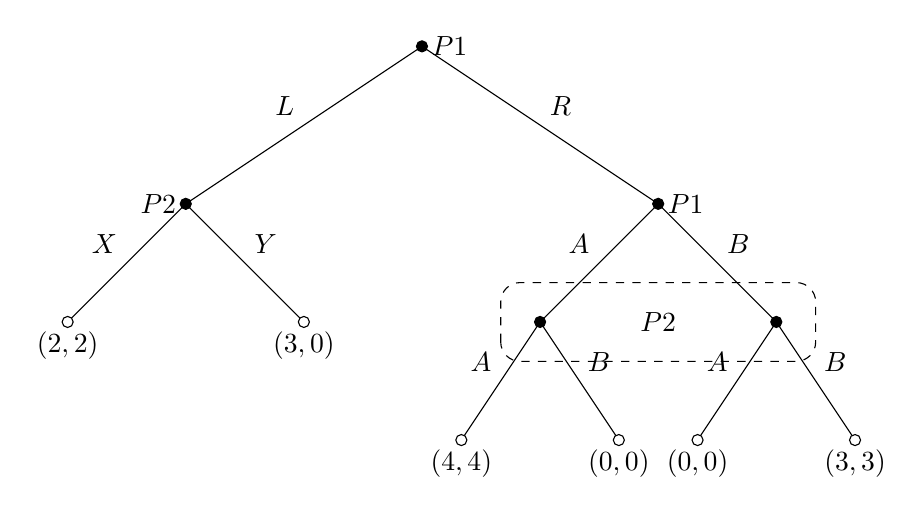
\begin{tikzpicture}
		\draw (-3,-2)--(0,0)--(3,-2);
		\draw (-4.5,-3.5)--(-3,-2)--(-1.5,-3.5);
		\draw (4.5,-3.5)--(3,-2)--(1.5,-3.5);
		\draw (2.5,-5)--(1.5,-3.5)--(0.5,-5);
		\draw (3.5,-5)--(4.5,-3.5)--(5.5,-5);
		\filldraw[color=black, fill=black] (0,0) circle(2pt);
		\filldraw[color=black, fill=black] (-3,-2) circle(2pt);
		\filldraw[color=black, fill=black] (3,-2) circle(2pt);
		\filldraw[color=black, fill=black] (1.5,-3.5) circle(2pt);
		\filldraw[color=black, fill=black] (4.5,-3.5) circle(2pt);
		\filldraw[color=black, fill=white] (5.5,-5) circle(2pt);
		\node[below] at (5.5,-5) {$(3,3)$};
		\filldraw[color=black, fill=white] (3.5,-5) circle(2pt);
		\node[below] at (3.5,-5) {$(0,0)$};
		\filldraw[color=black, fill=white] (2.5,-5) circle(2pt);
		\node[below] at (2.5,-5) {$(0,0)$};
		\filldraw[color=black, fill=white] (0.5,-5) circle(2pt);
		\node[below] at (0.5,-5) {$(4,4)$};
		\filldraw[color=black, fill=white] (-4.5,-3.5) circle(2pt);
		\node[below] at (-4.5,-3.5) {$(2,2)$};
		\filldraw[color=black, fill=white] (-1.5,-3.5) circle(2pt);
		\node[below] at (-1.5,-3.5) {$(3,0)$};
		\draw [dashed, rounded corners = 7] (1,-4) rectangle ++(4,1);
		\node[right] at (0,0) {$P1$};
		\node[left] at (-3,-2) {$P2$};
		\node[right] at (3,-2) {$P1$};
		\node at (3,-3.5) {$P2$};
		\node[above left] at (-1.5,-1) {$L$};
		\node[above left] at (-3.75,-2.75) {$X$};
		\node[above left] at (2.25,-2.75) {$A$};
		\node[above] at (0.75,-4.25) {$A$};
		\node[above] at (3.75,-4.25) {$A$};
		\node[above right] at (1.5,-1) {$R$};
		\node[above right] at (3.75,-2.75) {$B$};
		\node[above right] at (-2.25,-2.75) {$Y$};
		\node[above ] at (2.25,-4.25) {$B$};
		\node[above ] at (5.25,-4.25) {$B$};
	\end{tikzpicture}
\end{figure}

\begin{itemize}
	\item[(a)] List all pure strategies that each player has.
	\item[(b)] How many subgames are there? Please describe them.
	\item[(c)] Find all (pure or mixed) subgame-perfect equilibria.
	\item[(d)] Find a Nash equilibrium that is not subgame-perfect.
\end{itemize}

\paragraph{Solutions}.

\begin{itemize}
	\item[(a)] Player 1 has the strategies  $\{L,R\} \times \{A,B\}$. Player 2 has the strategies $\{X,Y\} \times \{A,B\}$.
	\item[(b)] Recall that a subgame begins at any non-terminal history. There are four subgames: one starting at the initial node, which is (trivially) the exact same as the original dynamic game in extensive form; one starting with Player 2's choice after Player 1 chooses $L$; one starting with Player 1's choice of $A$ or $B$ given that they have chosen $R$; and finally one starting with Player 2's choice of $A$ or $B$ given that Player 1 has chosen $R$.
	\item[(c)] Observe that $Y$ is strictly dominated for Player 2 in the subgame starting after Player 1 chooses $L$. The pure SPEs are $(RA,XA)$ and $(RB,XB)$. Finally, the other strategy is the unique mixed strategy of the $(A,B)$ subgame, where Player 1 plays $(L, 3/7 A + 4/7 B)$ and Player 2 plays $(X, 3/7 A + 4/7 B)$.
	\item[(d)] 
\end{itemize}


\section{Feb 28}

\subsection{Review}

\begin{model}
	The Rubinstein Bargaining Model involves two player $N = \{1,2\}$ who bargain over a pie of size 1, with individual discount factors $\delta_1,\delta_2$. In even periods $t$, player 1 offers $(\alpha_1,1-\alpha_1)$, and player 2 accepts or rejects. If they accept, the payoffs are $(\delta_1^t \alpha_1,\delta_2^t(1-\alpha_1))$. If they reject, play moves to the next period. In odd periods $t$, player 2 offers $(\alpha_1,1-\alpha_2)$ and player 1 accepts or rejects. If they accept, payoffs are $(\delta_1^t (1-\alpha_2),\delta_2^t\alpha_2)$. If they reject, the game moves to the next period.
\end{model}

\begin{definition}
	A strategy is stationary if the criterion for accepting or rejecting does not change period by period.
\end{definition}

\begin{remark}
	In stationary strategies, the unique subgame perfect equilibrium is \[(\alpha_i,1-\alpha_i) = \parl \frac{1-\delta_j}{1-\delta_i\delta_j}, \frac{\delta_j - \delta_i\delta_j}{1-\delta_i\delta_j}\parr\]Note that (i) there is immediate agreement, which is Pareto efficient, (ii) there is a first-mover advantage, and (iii) the more patient you are the better off you are.
\end{remark}

\begin{proposition}
	Consider a two-player infinite horizon bargaining game and a stationary strategy profile where player $i$ offers $(\alpha_i,1-\alpha_i)$ and accepts offers above the threshold $(1-\alpha_{-i})$. For any partial history where $i$ is the acceptor, let $z_i$ denote her expected payoff were play to continue to the next round. Additionally, let $w_i$ denote her expected payoff when $i$ is the offerer. Then the strategy profile is a subgame perfect Nash equilibrium if and only if $z_i = 1-\alpha_{-i}$ and $\alpha_i \ge w_i$.
\end{proposition}
\begin{proof}
	Direct, by the one-shot deviation principle.
\end{proof}

\subsection{Exercises}

\textbf{Question.}
Consider the same game as above, except at the beginning of every period a coin is tossed. If it comes up Heads, player 1 makes the offer. If it comes up tails, player 2 makes the offer.

\begin{enumerate}
	\item Assume first that the players agree that the probability of heads is $p\in (0,1)$. Find a subgame perfect equilibrium.
	\item Now assume that player $1$ believes that the probability of heads is $p_1 \in (0,1)$, and player 2 believes that the probability of tails is $p_2 \in (0,1)$. This disagreement is commonly known. Find a subgame perfect Nash equilibrium.
\end{enumerate}

\textbf{Answers.}

\begin{enumerate}
	\item Observe that our equilibrium is precisely characterized by four total conditions, involving the acceptance. We need, for strategies $(\alpha_i,1-\alpha_i)$ for $i \in \{1,2\}$ to be a subgame perfect equilibrium, that for any alternative $(\beta_1,\beta_2)$, that\begin{align*} (1-\alpha_2) &\ge p \delta \alpha_1 + (1-p)\delta (1-\alpha_2) &&(1 \text{ accepts}) \\ (1-\beta_2) &\le p \delta \alpha_1 + (1-p)\delta (1-\alpha_2) \forall \beta_2 > \alpha_2 &&(1 \text{ rejects}) \\ (1-\alpha_1) &\ge p \delta \alpha_2 + (1-p)\delta (1-\alpha_1) &&(2 \text{ accepts}) \\ (1-\beta_1) &\le p \delta \alpha_2 + (1-p)\delta (1-\alpha_1) \forall \beta_1 > \alpha_1 &&(2 \text{ rejects}) \end{align*}Which gets us the equations\[(1-\alpha_2 ) = p\delta \alpha_1 + (1-p)\delta (1-\alpha_2) \]and \[(1-\alpha_1) = p\delta \alpha_2 + (1-p)\delta (1-\alpha_1)\]which together characterize that \[\alpha_1 = 1-\delta + p\delta \qquad ; \qquad \alpha_2 = 1-p\delta\]
	\item We can solve this in the same way as part 1, and get the (somewhat tedious) characteriztion equations \[(1-\alpha_2) = p_1\delta \alpha_1 + (1-p_1)\delta (1-\alpha_2)\]and \[(1-\alpha_1) = p_2\delta \alpha_2 + (1-p_2) \delta (1-\alpha_1)\]which gets us\[\alpha_1 = \frac{1-\delta+p_1\delta}{(p_1+p_2)\delta - \delta + 1} \qquad ; \qquad \alpha_2 = \frac{1-\delta+p_2\delta}{(p_1+p_2)\delta - \delta + 1}\]
\end{enumerate}

\section{March 7}

\subsection{Review}

\begin{definition}
	A repeated game consists of (i) a set of players $N = \{1,\dots,n\}$; (ii) a set of actions for each player $A_i$; (iii) $T+1$ stages, where $T$ can be infinite; (iv) payoff functions in the stage game for each player; $g_i: A \to \reals$; (v) a discount factor $\delta \in (0,1]$; (vi) period-$t$ history $h^t = (a^0,a^1,\dots,a^{t-1})$; (vii) set of period-$t$ histories $\mathcal{H}^t = \{h^t\}$, with terminal histories $Z$; (viii) period-$t$ strategy $s_i^t: \mathcal{H}^t \to \Delta(A_i)$, where strategy $s_i = \{s_i^t\}_{t=0}^T$; (ix) a payoff function for finitely repeated games $u_i: Z \to \reals$ defined by \[u_i(s_i,s_{-i}) = \frac{1-\delta}{1-\delta^{T+1}} \sum_{t=0}^T \delta^t g_i(s_i(h^t),s_{-i}(h^t))\] and (x) a payoff function for infinitely repeated games $u_i:Z \to \reals$, where \[u_i(s_i,s_{-i}) = (1-\delta) \sum_{t=0}^\infty \delta^t g_i(s_i(h^t),s_{-i}(h^t))\]
\end{definition}

\begin{theorem}
	In an infinitely repeated game, a strategy $s$ is an SPE if and only if for all players $u$, all histories $h \in \mathcal{H}$, and one-stage deviations $\hat{s}_i$,\[u_i(s_i\mid_h , s_{-i} \mid_h) \ge u_i(\hat{s}_i,s_{-i}\mid_h)\]
\end{theorem}

\begin{proposition}
	Let $\alpha$ be a Nash equilibrium of the stage game. Consider the strategy profile $s$ such that for all $i$ and all $h^t$, $s_i(h^t) = \alpha$. Then $s$ is a subgame perfect equilibrium.
\end{proposition}

\begin{proposition}
	Suppose that $T < \infty$. If the stage game has a unique Nash equilibrium, then the repeated game has a unique SPE, which is repeating the Nash equilibrium in each stage game.
\end{proposition}

\begin{proposition}
	In the infinitely-repeated Prisoner's Dilemma, for sufficiently large $\delta$ the following strategy defines a symmetric SPE:\[s_i(h^t) = \begin{cases} C & h^t = ((C,C),\dots,(C,C))\\ C & t = 0 \\ D & \text{otherwise}\end{cases}\]
\end{proposition}
\begin{proposition}
	In the infinitely-repeated Prisoner's Dilemma, for $\delta \ge \frac{1}{2}$ there exists $T$ such that the following strategy defines a symmetric SPE:\[s_i(h^t) = \begin{cases} C & t = 0, (C,C) \text{ was played at } t-1, \text{ or } (D,D) \text{ was played from } t-T-1 \text{ to } t-1 \\ D & \text{otherwise}\end{cases}\]
\end{proposition}
\begin{proposition}
	In the infinitely repeated Prisoner's Dilemma, for $\delta = \frac{1}{2}$ the following strategy defines a symmetric SPE: \[s_i(h^t) = \begin{cases} C & t = 0 \\ C & s_{-i}(h^{t-1}) = C \\ D & \text{otherwise} \end{cases}\]
\end{proposition}


\subsection{Exercises}

Consider an infinitely repeated game where the stage game is a game of chicken:
\begin{center}
	\begin{tabular}{c|cc}
		& Swerve & Straight \\\hline 
		Swerve & $(0,0)$ & $(-1,1)$ \\
		Straight & $(1,-1)$ & $(-10,-10)$
	\end{tabular}
\end{center}
Assume that the discount factor is close to 1. For concreteness, you may assume $\delta = 0.99$.

\begin{enumerate}
	\item Is there an SPE in which player 1's payoff is $\frac{1}{1-\delta}$? Explain
	\item Is there an SPE in which each player's payoff is $0$? Explain
	\item Is there an SPE in which player 1's payoff is $-\frac{2}{1-\delta}$? Explain
\end{enumerate}

\section{March 14}

\subsection{Review} 

\begin{definition}
	The set of feasible payoffs is the convex hull of payoffs generated by the pure action profiles in the stage game.
\end{definition}
\begin{definition}
	Player $i$'s minimax payoff is \[\underline{v}_i = \min_{s_{-i}} \barl \max_{s_i} g_i(s_i,s_{-i})\barr\]where $s_i$ and $s_{-i}$ are mixed strategies.
\end{definition}

\begin{remark}
	This is the lowest payoff player $i$'s opponent can hold him to by any choice of $s_{-i}$, provided that player $i$ correctly foresees $s_{-i}$ and plays a best response to it.
\end{remark}
\begin{theorem}
	\emph{Nash Folk Theorem} For every payoff vector $v$ with $v_i > \underline{v}_i$ for each player $i$, there exists $\underline{\delta}<1$ such that for all $\delta \in (\underline{\delta},1)$, there is a Nash equilibrium of $G_\infty(\delta)$ with payoff $v$.
\end{theorem}
\begin{theorem}
	\emph{Nash Threats Folk Theorem} Let $\alpha\opt$ be a Nash equilibrium of the stage game with payoffs $e$. Then for every feasible payoff vector $v$ with $v_i > e_i$ for all $i$, there exists $\underline{\delta}<1$ such that for all $\delta \in (\underline{\delta},1)$, there is a \textbf{subgame perfect} Nash equilibrium of $G_\infty(\delta)$ with payoff $v$.
\end{theorem}
\begin{theorem}
	\emph{SPE Folk Theorem} Assume that the dimension of the set of feasible payoffs is equal to the number of players. Then for any $v$ with $v_i > \underline{v}_i$ for all $i$, there exists $\underline{\delta} < 1$ such that for all $\delta \in (\underline{\delta},1)$, there is a subgame perfect Nash equilibrium of $G_\infty(\delta)$ with payoff $v$.
\end{theorem}



\section{March 28}

\subsection{Review}

\begin{definition}
	We have a set of $N$ players, a finite set of states of nature $\Omega$, and for each $i \in N$; (i) an action set $A_i$; (ii) a set of types $T_i$ and a signal function $\tau_i: \Omega \to T_i$; (iii) a probability measure $p_i$ over $\Omega$; and (iv) a preference relation $\succeq_i$ over $A \times \Omega$.
\end{definition}

\begin{definition}
	A Bayesian Nash Equilibrium is the Nash equilibrium of the strategic game where the set of players is the set $(i,t_i)$ for $i \in N$, $t_i \in T_i$; the set of actions for player $(i,t_i)$ is $A_i$; and the preferences of $(i,t_i)$ are defined as \[a\opt \succeq b\opt \iff L_i(a\opt,t_i) \succeq L_i(b\opt,t_i)\]where $L_i$ is a lottery over $A \times \Omega$ that assigns probability $\frac{p_i(\omega)}{p_i(\tau_i^{-1}(t_i))}$ to $(a_{\tau_j(\omega)},\omega)$ if $\omega \in \tau_i^{-1}(t_i)$ and 0 otherwise.
\end{definition}

\begin{definition}
	In a Bayesian game, each player and type has a strategy. Equivalently, we can say that player $i$'s strategy is a function that maps her type to her action: $\sigma_i: T_i \to \Delta(A_i)$. Let $\sigma(t) = (\sigma_1(t_1),\dots,\sigma_N(t_N))$ denote the strategy profiles. Player $i$'s expected payoff from playing $a_i$ when receiving signal $t_i$ is \[u_i(a_i,\sigma_{-i}\mid t_i) = \sum_{\omega,t_{-i}} u_i(\omega,a_i,\sigma_{-i}(t_{-i}))p(\omega,t_{-i}\mid t_i)\]So a strategy profile $\sigma$ is a Bayesian Nash Equilibrium if and only if for all $i$, $t_i$, and $a_i$ such that $\sigma_i(a_i \mid t_i)> 0$\[u_i(a_i,\sigma_{-i}\mid t_i) = \max_{a_i'}u_i(a_i',\sigma_{-i}\mid t_i)\]
\end{definition}







\end{document}